\section{Introduction}

%title page
\begin{frame}
\titlepage
\end{frame}

\begin{frame}{Introduction: \\The astroparticle physics data rate}
%или "Астрофизика - современное состояние"))
\small
\begin{columns}
  \begin{column}[t]{0.45\textwidth}
    \begin{center}
      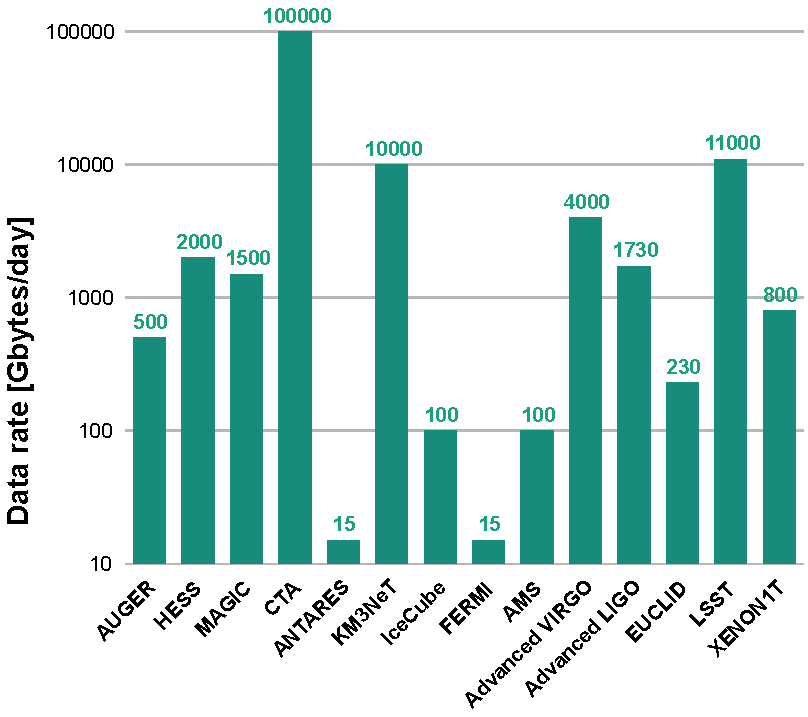
\includegraphics[width=1\textwidth]{pics/appec_base4.pdf}
    \end{center}
    \vspace{-2\parsep}
    \small Modern astroparticle experiments data rate [Gbytes/day]\footnotemark[1] %, source: APPEC brochure on Computing, 2016}
  \end{column}
  \hfill
  \begin{column}[t]{0.53\textwidth}
    % \vspace{1.5em}
    % Вступление - такие вступление :)
    % Современная астрофизика представлена большим количеством экспериментов, которые изучают примерно одно и то же (а зачастую - и прям совсем одно и то же, в плане объекта), но по-разному - т.е., в разных природных условиях и с использованием разных типов детекторов.
    % Каждый год данных прибывает, и при этом общй дата пул ежегодно растет, как на дрожжах (см. картинку)
    \begin{itemize}
    \item Wide range of experiments;
    \item Looking at the same sky with different eyes: different detectors, different phenomena under the study;
    \item Common data rate for astrophysical experiments all together is a few PBytes/yeary, which is comparable to the current LHC output\footnotemark[1] % \textcolor{red}{(ссылка на брощюру!!!)}
    \item Big data for deep learning
    %\ldots
%     \item Need for collaboration
    \end{itemize}

%     \textcolor{red}{TODO: дописать текста, чтобы сбалансирвоать дизайн страницы}
  \end{column}
\end{columns}
  \footnotesize\footnotetext[1]{APPEC brochure on Computing, 2016}
\end{frame}

% \begin{frame}{\textcolor{kit-green100}{KRAD}: \textcolor{kit-green100}{K}arlsruhe-\textcolor{kit-green100}{R}ussian \textcolor{kit-green100}{A}stroparticle \textcolor{kit-green100}{D}ata Life Cycle}
\begin{frame}{German-Russian Astroparticle Data Life Cycle}
\vspace{-1.4em}
% \textcolor{red!50!black}{Change the collboration picture}
\begin{center}
  
\includegraphics[width=0.9\textwidth]{pics/Collab.eps}
\end{center}
% \vspace{-2\parsep}
% The first Russian-German big data collaboration

\vspace{-1em}
% \footnotesize
% \begin{itemize}
%   \setlength{\itemsep}{0pt}
%   \item Minh Duc Nguyen, \textit{A distributed data warehouse system for astroparticle physics}, GRID2018 session 10
%   \item Yu. Kazarina, \textit{Application of Hubzero platform for the educational process in astroparticle physics}, GRID2018 poster session
% \end{itemize}
\end{frame}

\begin{frame}{KASCADE}
\begin{itemize}
  \item Proposed in 1989---disassembled in 2013;
  \item Aimed at studying processes at the edge of the Galaxy and beyond by observing extended atmospheric showers (EAS);
  \item Consisted of:
  \begin{itemize}
    \item scintillators detecting $e$, $\gamma$, $\mu$:
    \begin{itemize}
  %сцинтиляторы, различают e, gamma, mu
    \item KASCADE - 256 stations;
    \item GRANDE - 37 stations;
    \end{itemize}
 %один большой калориметр
    \item Hadronic callorimeter;
 %радиодетектор
    \item Radiodetector LOPES detecting $e$, $e^{+}$;
% позволяющих наблюдать различные компоненты ливня
  \end{itemize}
  \item Recognized astrophysical results were obtained. The data analysis is ongoing;
%  благодаря данным с эксперимента было открыто много всего ополезного, при этом анлиз данных продолжается. новые статьи выходят
  \item KCDC (\textbf{K}ASCADE \textbf{C}osmic Ray \textbf{D}ata \textbf{C}enter, \textcolor{blue}{\texttt{http://kcdc.ikp.kit.edu}}) is a dedicated portal where all the data collected are available online. % At the moment
%   к настоящему времени все данные эксперимента опубликованы и доступны онлайн, для этих целей был сделан
%  принциально принципиально новый и крутой на тот момент портал KCDC
% \textcolor{red!50!black}{Add the kcdc logo in the center of the slide}
\end{itemize}

\parbox[t][0pt]{0pt}{
  \vspace{-0.63\textheight}
  ~\hspace{0.68\textwidth}
\includegraphics[width=0.3\textwidth]{pics/KCDC-logo.png}
}
\end{frame}

\begin{frame}{TAIGA}
\footnotesize
\vspace{-1em}
\begin{itemize}
 \item Started in the mid 90s and still operating
%  \item Currently consists of 4 detectors presented + TUNKA IACT is under construction;
\end{itemize}
\vspace{-2em}
\begin{minipage}[t]{0.31\textwidth}
  \begin{block}{\small Tunka-133}
    \parbox[c][0.20\textheight][t]{1\textwidth}{
      \centering
      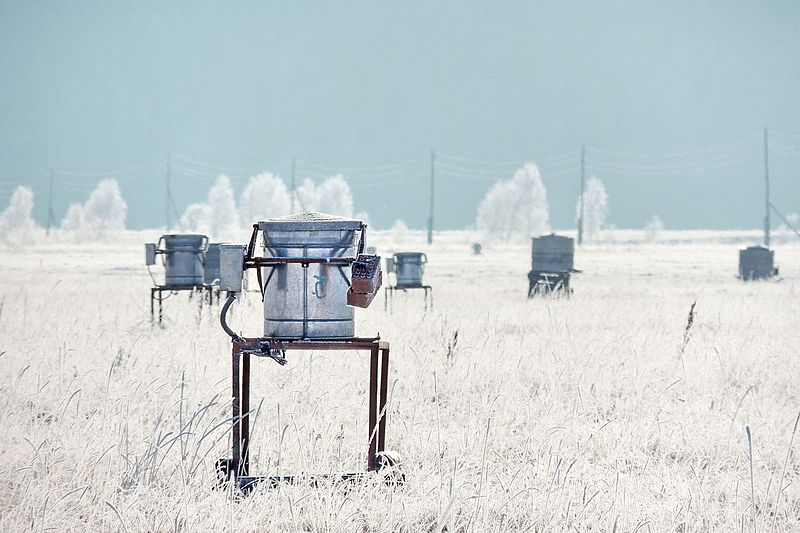
\includegraphics[width=0.7742\textwidth]{pics/Tunka-133.jpg}
    }
    \hfill
    \parbox[c][0.15\textheight][t]{1\textwidth}{
      \begin{itemize}
        \setlength{\itemsep}{0pt}
        \item 133 photomultipliers
        \item measures EAS Cherenkov light
      \end{itemize}
    }
  \end{block}
\end{minipage}
\hfill
\begin{minipage}[t]{0.31\textwidth}
  \begin{block}{\small Tunka-Rex}
    \parbox[c][0.20\textheight][t]{1\textwidth}{
      \centering
      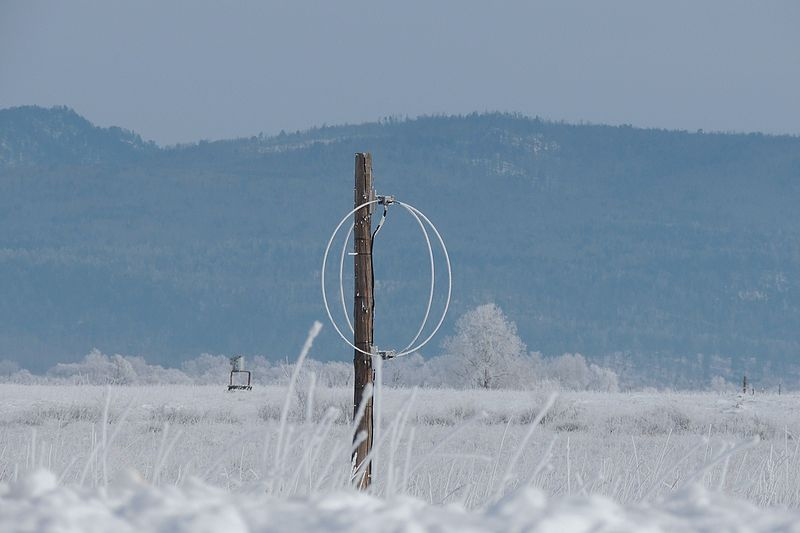
\includegraphics[width=0.7742\textwidth]{pics/Tunka-Rex.jpg}
    }
    \\
    \parbox[c][0.15\textheight][t]{1\textwidth}{
      \begin{itemize}
        \setlength{\itemsep}{0pt}
        \item 63 antennas
        \item measures EAS radio-emission
      \end{itemize}
    }
  \end{block}
\end{minipage}
\hfill
\begin{minipage}[t]{0.31\textwidth}
  \begin{block}{\small Tunka-HiSCORE}
    \parbox[c][0.20\textheight][t]{1\textwidth}{
      \centering
      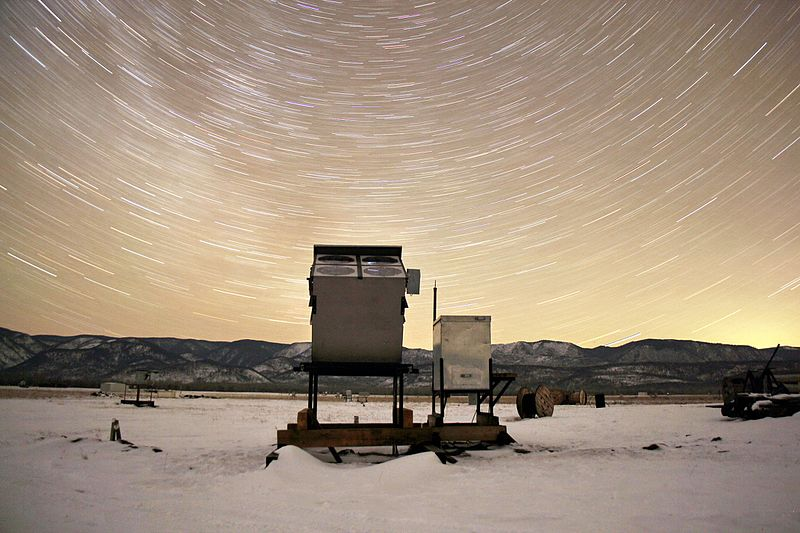
\includegraphics[width=0.7742\textwidth]{pics/Tunka-HiSCORE.jpg}
    }
    \\
    \parbox[c][0.15\textheight][t]{1\textwidth}{
      \begin{itemize}
        \setlength{\itemsep}{0pt}
        \item 47 photomultipliers
        \item measures EAS Cherenkov light
      \end{itemize}
    }
  \end{block}
\end{minipage}

\vspace{-1ex}
\begin{minipage}[t]{0.48\textwidth}
  \begin{block}{\small Tunka-Grande}
    \parbox[c][0.21\textheight][t]{0.43\textwidth}{
      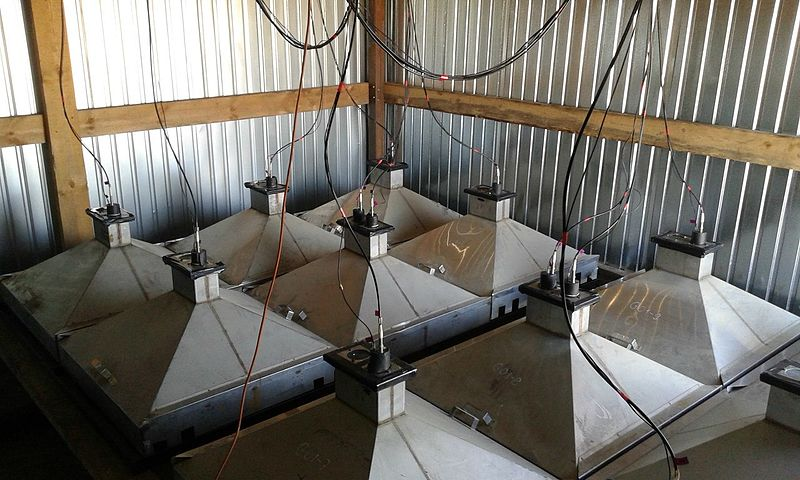
\includegraphics[width=0.50\textwidth]{pics/Hiller_Roman-005.jpg}
    }
    \hfill
    \parbox[c][0.21\textheight][t]{0.55\textwidth}{
      \begin{itemize}
        \setlength{\itemsep}{0pt}
        \item 380 scintillators 0.64m$^2$ each
        \item measures $e$/$\mu$ from EAS
      \end{itemize}
    }
  \end{block}
\end{minipage}
\hfill
\begin{minipage}[t]{0.48\textwidth}
  \begin{block}{\small Tunka-IACT}
    \parbox[c][0.21\textheight][t]{0.43\textwidth}{
      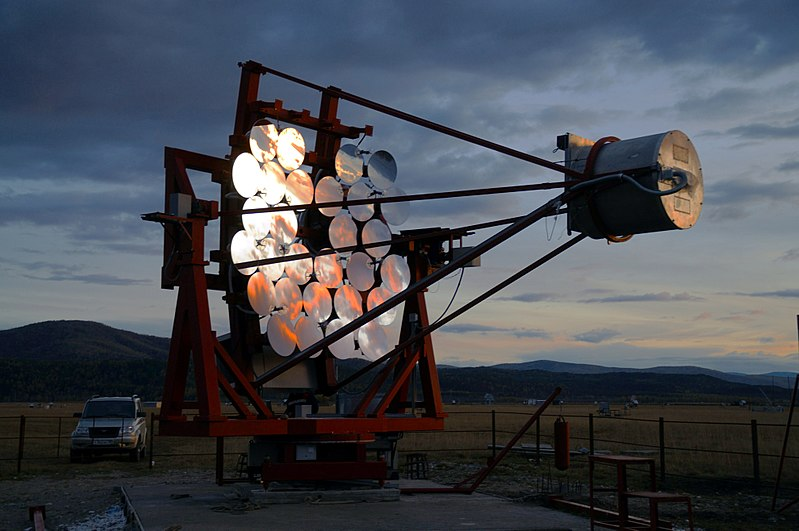
\includegraphics[width=0.50\textwidth]{pics/Tunka-Iact.jpg}
    }
    \hfill
    \parbox[c][0.21\textheight][t]{0.55\textwidth}{
      \begin{itemize}
        \setlength{\itemsep}{0pt}
        \item Imaging Air Cherenkov Telescopes
        \item is being extended
      \end{itemize}
    }
  \end{block}
\end{minipage}
\end{frame}

%
% \begin{frame}
%  \begin{exampleblock}{title}
%   text
%  \end{exampleblock}
%
% \end{frame}
